\documentclass[12pt]{article}

\usepackage[margin=2cm]{geometry}

\usepackage[utf8]{inputenc}
\usepackage[T1]{fontenc}

%% Loading tcolorbox for easy laying out of
%% LaTeX code and output side-by-side
\usepackage{xcolor}
\usepackage{tcolorbox}
\tcbuselibrary{minted}
\newtcblisting{mybox}{colback=white,minted language=latex,listing side text,righthand width=.2\textwidth}

\usepackage{tikzducks}

\begin{document}

\begin{mybox}
% A basic duck
\tikz\duck;
\end{mybox}


\begin{mybox}
% An Overleaf duck!
\tikz\duck[overleaf];
\end{mybox}


\begin{mybox}
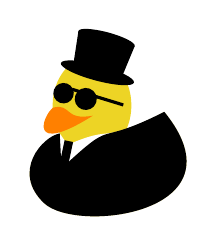
\begin{tikzpicture}
%% Accessorise -- be smart!
\duck [tshirt=white, jacket=black, tie=black, tophat=black, 
  sunglasses=black, bill=orange];
\end{tikzpicture}
\end{mybox}


\begin{mybox}
%% DISCO!!

\begin{tikzpicture}
\duck[eyebrow, mullet=black, jacket=white,
  lapel=black, buttons=gray!20, bill=orange,
  necklace=orange!80!yellow, speech={\footnotesize\sffamily Disco}
];
%% Sometimes you may need to draw extra paths
\path[draw]\duckpathjacket;
\path[draw,xshift=12pt,fill=white]\duckpathwing;
\end{tikzpicture}
\end{mybox}


\begin{mybox}
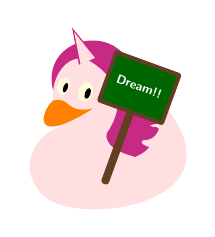
\begin{tikzpicture}
\duck [body=pink!50!white,bill=orange,
  unicorn=magenta!60!violet, longhair=magenta!60!violet,
  signpost=\scalebox{0.45}{%
     \parbox{4em}{\sffamily\bfseries\centering Dream!!}}
      ]
\end{tikzpicture}
\end{mybox}

\end{document}
